\chapter{Description du modèle à réaliser}\label{ch:papud_model}
Le modèle à réaliser est conçu pour être le plus rapide possible.

Le modèle est un \gls{lm} au niveau du caractère, qui prend en entrée une ligne et qui prédit la ligne suivante.

Ainsi, l'entrée du modèle est une ligne de taille fixe de nombres correspondant à des caractères.

La sortie est un tableau à 2 dimensions, qui contient pour chaque caractère prédit une distribution de probailité sur les caractères connus (répertoriés dans le dictionnaire décrit \autoref{def_dict_papud}, \autopageref{def_dict_papud}).

\section{Utilisation d'un \glsentrytext{nn} basique}
Comme présenté dans le \autoref{ch:project_papud} (\autopageref{ch:project_papud}), un \gls{nn} basique, intégralement connecté, a été choisi pour le modèle.

Étant le \gls{nn} le plus simple, il est extrêmement rapide à entraîner.

\section{Réduction de la taille de l'entrée}
Comme écrit plus haut, l'entrée du modèle est une ligne de caractères.
Pour chacun d'entre eux, comme dans le modèle \gls{gmsnn}, est transformé en un \gls{tensor} par un module d'\gls{embedding} (voir la \autoref{def:embedding}, \autopageref{def:embedding}).

Grâce à une opération appelée \og \foreign{max-pooling} \fg{}, qui correspond à prendre pour chaque case du \gls{tensor} final la valeur maximale des cases correspondantes des \glspl{tensor} initiaux.

Par exemple~:
\[ \text{max-pool}\left(\left[\begin{array}{ccc}0&30&6\\-5&6&12\end{array}\right] , \left[ \begin{array}{ccc}2&42&3\\5&-60&-2\end{array}\right] \right) = \left[\begin{array}{ccc}2&42&6\\5&6&12\end{array}\right]  \]

Car $0<2$, $30<42$, $6>3$, $-5<5$, $6>-60$ et $12>-2$.

\section{Représentation de l'architecture}

La façon dont s'agencent les différents modules de l'architecture est représentée dans la \autoref{fig:base_papud} (\autopageref{fig:base_papud}).

\begin{figure}[ht]
	\centering
	\usetikzlibrary{calc}

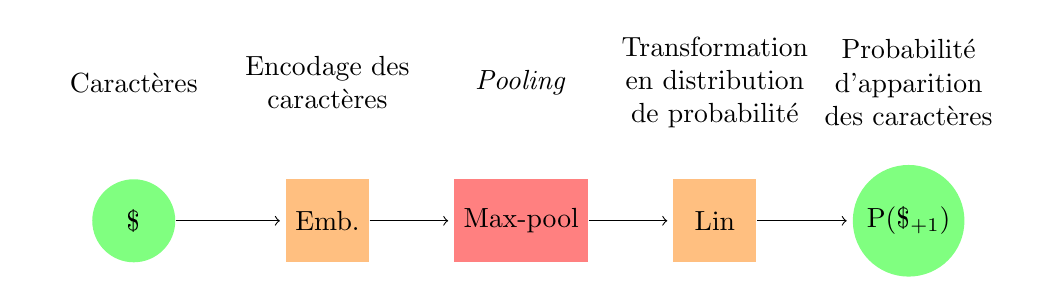
\begin{tikzpicture}[shorten >=2pt,->,draw=black, node distance=7em]
    \tikzstyle{every pin edge}=[<-,shorten <=2pt]
	\tikzstyle{module}=[minimum size=3em, fill=gray!50!]
	\tikzstyle{char}=[module, circle, fill=green!50!]%, label={below:\usebox\mydictbox}]
	\tikzstyle{text label}=[rectangle, text centered, text width=7em, node distance=5em]
	\tikzstyle{nn}=[rectangle, module, fill=orange!50!]
	\tikzstyle{rnn}=[nn, fill=red!50!]

	\node[char] (char) {\$};
	\node[nn, right of=char] (emb) {Emb.};
	\node[rnn, right of=emb] (rnn) {Max-pool};
	%\draw[->] (rnn.north) to [out=90,in=90, looseness=2] ($(rnn.west) + (-0.5,0)$) to [out=-90,in=-90, looseness=2] (rnn.south);
	\node[nn, right of=rnn] (lin) {Lin};
	\node[char, right of=lin] (out) {P(\$$_{+1}$)};
	\draw[->] (char) to (emb);
	\draw[->] (emb) to (rnn);
	\draw[->] (rnn) to (lin);
	\draw[->] (lin) to (out);
	%\node[char] (char) {\$};


    \node[text label, above of=char] (charl) {Caract\`{e}res};
    \node[text label, above of=emb] (embl) {Encodage des caract\`{e}res};
    \node[text label, above of=rnn] (rnnl) {\textit{Pooling}};
    \node[text label, above of=lin] (linl) {Transformation en distribution de probabilit\'{e}};
    \node[text label, above of=out] (outl) {Probabilit\'{e} d'apparition des caract\`{e}res};
\end{tikzpicture}
	\caption[Architecture du modèle du projet PAPUD]{Architecture du modèle du \gls{project_papud}}
	\label{fig:base_papud}
\end{figure}

\section{Lien avec l'état de l'art}
Il a été récemment montré que les \gls{lm} simples basés sur des  \glspl{embedding} et des opération de \foreign{pooling}
montre des performances équivalentes voir supérieures à des modèles plus complexes et plus coûteux comme les \gls{rnn} \autocite{pooling_simple}.

%%%%%%%%%%%
%
%Modèle ultra-rapide au niveau caractere:
%
%un embedding par caractere
%embedding de la ligne = max-pool des embeddings des caracteres
%
%
%Training: predire X_{t+d}
%
%plutot que d'utiliser un RNN pour generer X_{t+d} (trop lent), on accelere en generant avec un simple fully-connected
%une ligne de taille fixe (il faudra pad/cut)